\documentclass[12pt]{scrartcl}

\usepackage[utf8]{inputenc}
\usepackage[IL2]{fontenc}
\usepackage[czech]{babel}
\usepackage{graphicx}
\usepackage{hyperref}
\usepackage{amsmath}
\usepackage[]{algorithm2e}
\usepackage{enumitem}

\subject{Západočeská univerzita v\nobreakspace Plzni\\Fakulta aplikovaných věd\\KIV/KPG}
\author{Pavel Zelenka\\A16B0176P\\zelenkap@students.zcu.cz}
\date{\today}
\title{Triomino}

\begin{document}
\maketitle
\pagenumbering{gobble}
\newpage
\pagenumbering{arabic}
\newpage
\section{Zadání}
	
\paragraph{}
Zadáním úkolu je vytvoření programu vykreslujícího dlaždicový vzor známý pod\nobreakspace pojmem polymino. Konkrétně polyomina třetího řádu, tzn. triomino.


\section{Analýza problému}

\paragraph{}
\textbf{Triomino} je polymino třetíto řádu. Mnohoúhelníky vyplňující plochu se\nobreakspace skládají ze\nobreakspace tří stejně velkých čtverců. Tyto stejně velké čtverce jsou\nobreakspace napojeny ve\nobreakspace tvaru tvořící symbol\nobreakspace \texttt{L}.

\section{Popis řešení}

\paragraph{}
Vykreslování probíhá ve\nobreakspace třídě \emph{Drawing}. Pro\nobreakspace vykreslení triomino se\nobreakspace zavolá metoda \emph{\mbox{drawTriomino}}, která na\nobreakspace základě velikosti okna a\nobreakspace velikosti mnohoúhelníku provede potřebný počet iterací pro\nobreakspace vyplnění celého okna. Vyplňování probíhá od\nobreakspace levého dolního rohu.

\paragraph{}
\begin{algorithm}[H]
	\While{není dosaženo pravého hornho okraje okna} {
		\For{další sloupec} {
			\For{další řádek} {
				\BlankLine
				nastav pozici vykreslování na další řádek a sloupec
				\BlankLine
				\If{sloupec = 0 a řádek (mod 4) = 0}{
					vykresli mnohoúhelník				
				}
				\If{sloupec (mod 4) = 0 a řádek = 0 a sloupec $\neq$ 0}{
					vykresli mnohoúhelník				
				}
				\If{sloupec (mod 4) = 2 a řádek = 0}{
					vykresli mnohoúhelník				
				}
				\If{sloupec = 0 a řádek (mod 4) = 2}{
					vykresli mnohoúhelník				
				}
				\If{sloupec = 1 a řádek (mod 4) = 0 a řádek $\neq$ 0}{
					vykresli mnohoúhelník				
				}
				\If{sloupec = 1 a řádek (mod 4) = 2 a řádek $\neq$ 2}{
					vykresli mnohoúhelník				
				}
				\If{sloupec (mod 4) = 0 a řádek = 1 a sloupec $\neq$ 0}{
					vykresli mnohoúhelník				
				}
				\If{sloupec (mod 4) = 2 a řádek = 1 a sloupec $\neq$ 2}{
					vykresli mnohoúhelník				
				}
				\If{sloupec = řádek}{
					vykresli mnohoúhelník				
				}
				\BlankLine
				obnov pozici vykreslování na původní pozici
				\BlankLine
			}
		}
		\BlankLine
			nastav řádek = 0 a sloupec = 0
		\BlankLine
		\BlankLine
			zmenši oblast na které probíha vykreslování o 3 velikosti mnohoúhelníku
		\BlankLine
	}
 \caption{Vykreslení mnohoúhelníků}
\end{algorithm}

\newpage
\section{Uživatelská dokumentace}

\paragraph{}
Spuštění aplikace se\nobreakspace provede souborem \texttt{Triomino.jar}, který se nachází ve složce \emph{App}.

\paragraph{}
Po\nobreakspace spuštění aplikace se\nobreakspace zobrazí okno, které bude vydlážděno vygenerovaným vzorem. Velikost dlaždic lze měnit kliknutím na tlačítka \texttt{+} a \texttt{-} v\nobreakspace pravém dolním rohu. Barvu dlaždic lze měnit v\nobreakspace levém dolním rohu, kde je přepínač barev.	

\begin{figure}[!ht]
	\centering
	\label{obr:polekolizi}
	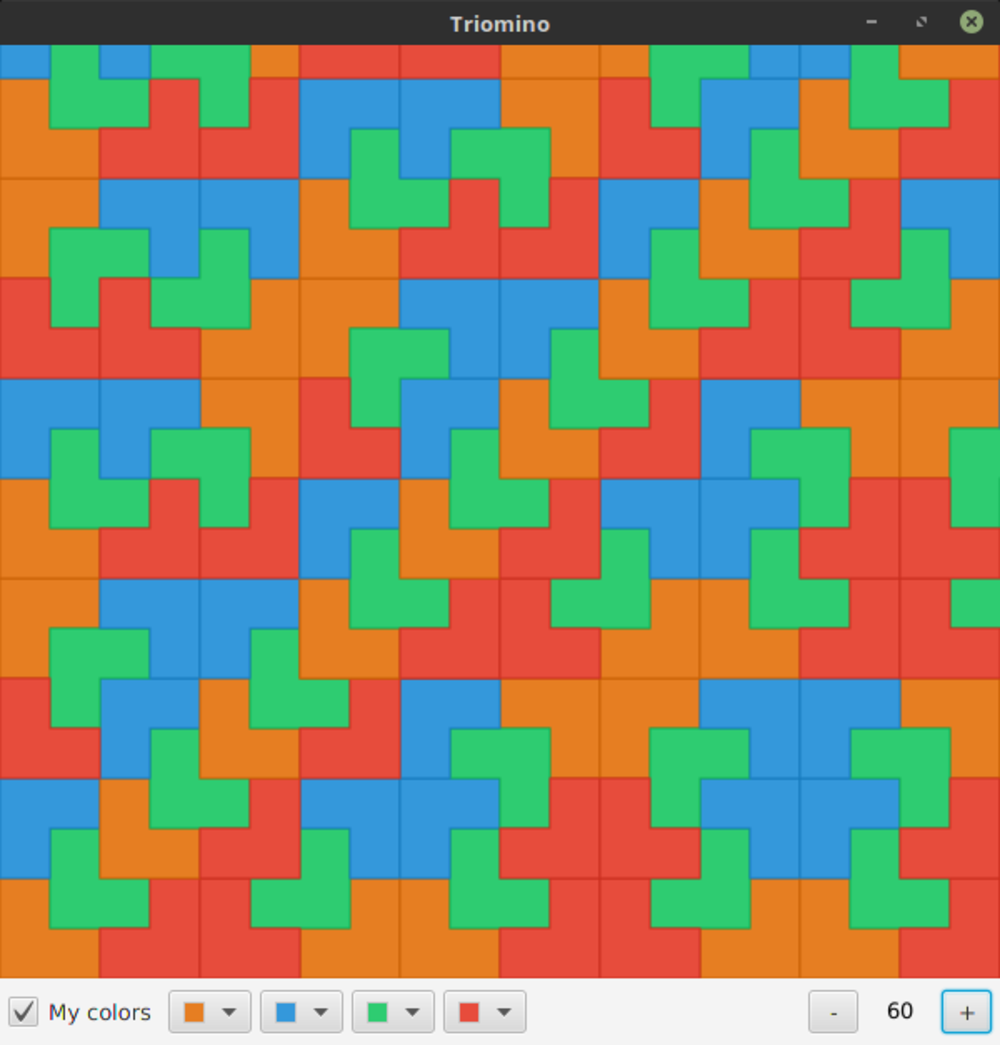
\includegraphics[width=0.8\textwidth,natwidth=1,natheight=1]{app_gui.pdf}
	\caption{Okno aplikace}
\end{figure}

\newpage
\section{Závěr}
\paragraph{}
Úkol jsem řešil v\nobreakspace jazyce \texttt{Java} s použitím grafických knihoven \texttt{JavaFX}.
Nejsem si\nobreakspace zcela jistý, zdali jsou dlaždice do sebe zapasovány v\nobreakspace požadovaném pořadí, zdá se\nobreakspace mi, že se\nobreakspace výsledek úplně neshoduje s\nobreakspace ilustrací v\nobreakspace zadání.

\section{Reference}

Tromino – Wikipedie. [online]. Dostupné z: \href{https://en.wikipedia.org/wiki/Tromino}{en.wikipedia.org/wiki/Tromino}

\end{document}
